% This is "sig-alternate.tex" V2.0 May 2012
% This file should be compiled with V2.5 of "sig-alternate.cls" May 2012
%
% This example file demonstrates the use of the 'sig-alternate.cls'
% V2.5 LaTeX2e document class file. It is for those submitting
% articles to ACM Conference Proceedings WHO DO NOT WISH TO
% STRICTLY ADHERE TO THE SIGS (PUBS-BOARD-ENDORSED) STYLE.
% The 'sig-alternate.cls' file will produce a similar-looking,
% albeit, 'tighter' paper resulting in, invariably, fewer pages.
%
% ----------------------------------------------------------------------------------------------------------------
% This .tex file (and associated .cls V2.5) produces:
%       1) The Permission Statement
%       2) The Conference (location) Info information
%       3) The Copyright Line with ACM data
%       4) NO page numbers
%
% as against the acm_proc_article-sp.cls file which
% DOES NOT produce 1) thru' 3) above.
%
% Using 'sig-alternate.cls' you have control, however, from within
% the source .tex file, over both the CopyrightYear
% (defaulted to 200X) and the ACM Copyright Data
% (defaulted to X-XXXXX-XX-X/XX/XX).
% e.g.
% \CopyrightYear{2007} will cause 2007 to appear in the copyright line.
% \crdata{0-12345-67-8/90/12} will cause 0-12345-67-8/90/12 to appear in the copyright line.
%
% ---------------------------------------------------------------------------------------------------------------
% This .tex source is an example which *does* use
% the .bib file (from which the .bbl file % is produced).
% REMEMBER HOWEVER: After having produced the .bbl file,
% and prior to final submission, you *NEED* to 'insert'
% your .bbl file into your source .tex file so as to provide
% ONE 'self-contained' source file.
%
% ================= IF YOU HAVE QUESTIONS =======================
% Questions regarding the SIGS styles, SIGS policies and
% procedures, Conferences etc. should be sent to
% Adrienne Griscti (griscti@acm.org)
%
% Technical questions _only_ to
% Gerald Murray (murray@hq.acm.org)
% ===============================================================
%
% For tracking purposes - this is V2.0 - May 2012

\documentclass{sig-alternate}

\usepackage{url}
\usepackage{xspace}

\newcommand{\psharp}{P\#\xspace}
\newcommand{\csharp}{C\#\xspace}

\usepackage{color}
\newcommand{\PDComment}[1]{\textcolor{cyan}{Pantazis: #1}}

\begin{document}
%
% --- Author Metadata here ---
\conferenceinfo{WOODSTOCK}{'97 El Paso, Texas USA}
%\CopyrightYear{2007} % Allows default copyright year (20XX) to be over-ridden - IF NEED BE.
%\crdata{0-12345-67-8/90/01}  % Allows default copyright data (0-89791-88-6/97/05) to be over-ridden - IF NEED BE.
% --- End of Author Metadata ---

\title{Uncovering Distributed System Bugs\\ during Testing (not Production!)}
%
% You need the command \numberofauthors to handle the 'placement
% and alignment' of the authors beneath the title.
%
% For aesthetic reasons, we recommend 'three authors at a time'
% i.e. three 'name/affiliation blocks' be placed beneath the title.
%
% NOTE: You are NOT restricted in how many 'rows' of
% "name/affiliations" may appear. We just ask that you restrict
% the number of 'columns' to three.
%
% Because of the available 'opening page real-estate'
% we ask you to refrain from putting more than six authors
% (two rows with three columns) beneath the article title.
% More than six makes the first-page appear very cluttered indeed.
%
% Use the \alignauthor commands to handle the names
% and affiliations for an 'aesthetic maximum' of six authors.
% Add names, affiliations, addresses for
% the seventh etc. author(s) as the argument for the
% \additionalauthors command.
% These 'additional authors' will be output/set for you
% without further effort on your part as the last section in
% the body of your article BEFORE References or any Appendices.

\numberofauthors{6} %  in this sample file, there are a *total*
% of EIGHT authors. SIX appear on the 'first-page' (for formatting
% reasons) and the remaining two appear in the \additionalauthors section.
%
\author{
% You can go ahead and credit any number of authors here,
% e.g. one 'row of three' or two rows (consisting of one row of three
% and a second row of one, two or three).
%
% The command \alignauthor (no curly braces needed) should
% precede each author name, affiliation/snail-mail address and
% e-mail address. Additionally, tag each line of
% affiliation/address with \affaddr, and tag the
% e-mail address with \email.
%
% 1st. author
\alignauthor Pantazis Deligiannis\\
       \affaddr{Imperial College London}\\
       \affaddr{London, UK}\\
       \email{p.deligiannis@imperial.ac.uk}
% 2nd. author
\alignauthor John Erickson\\
       \affaddr{Microsoft}\\
       \affaddr{Redmond, WA, USA}\\
       \email{jerick@microsoft.com}
% 3rd. author
\alignauthor Cheng Huang\\
       \affaddr{Microsoft Research}\\
       \affaddr{Redmond, WA, USA}\\
       \email{cheng.huang@microsoft.com}
\and  % use '\and' if you need 'another row' of author names
% 4th. author
\alignauthor Matt McCutchen\\
       \affaddr{MIT}\\
       \affaddr{Cambridge, MA, USA}\\
       \email{rmccutch@mit.edu}
% 5th. author
\alignauthor Shaz Qadeer\\
       \affaddr{Microsoft Research}\\
       \affaddr{Redmond, WA, USA}\\
       \email{qadeer@microsoft.com}
% 6th. author
\alignauthor Wolfram Schulte\\
       \affaddr{Microsoft}\\
       \affaddr{Redmond, WA, USA}\\
       \email{schulte@microsoft.com}
}

\date{17 August 2015}
% Just remember to make sure that the TOTAL number of authors
% is the number that will appear on the first page PLUS the
% number that will appear in the \additionalauthors section.

\maketitle
\begin{abstract}
Testing distributed systems is very challenging due to multiple sources of nondeterminism, such as arbitrary interleavings between event handlers and unexpected node failures. Stress testing, commonly used in industry today, is unable to deal with this kind of nondeterminism, which results in the most tricky bugs being missed during testing and only getting exposed in production.

We present a new methodology for systematically testing unmodified distributed systems. Our approach involves the use of \psharp, an extension of \csharp that combines a flexible environmental modeling approach with a concurrency testing framework, which can capture and systematically explore all sources of nondeterminism. We present two case studies of using \psharp to test production distributed systems inside Microsoft. Using \psharp, we managed to uncover a very subtle bug that was haunting developers for a long time, as they did not have an effective way to reproduce it. \psharp uncovered the bug in a very small setting, which made it easy to examine traces, identify and fix the problem.

\end{abstract}

\category{D.2.4}{Software Engineering}{Software/Program Verification}
\category{D.2.5}{Software Engineering}{Testing and Debugging}

\keywords{distributed systems, testing}

\section{Introduction}
\label{sec:intro}

Distributed systems are notoriously hard to test. This is due to many well-known sources of \emph{nondeterminism}, such as race conditions in the asynchronous interaction between system components, the use of multithreaded code inside a component, unexpected node failures, unreliable communication channels and message losses, and interaction with clients and external services.
%
All these sources of nondeterminism translate into \emph{exponentially} many execution paths that a distributed system might potentially execute. A bug might hide deep inside one of these paths and only manifest under extremely rare corner cases.

Classic techniques that product groups employ to test, verify and validate their systems (such as code reviews, stress testing, fault injection, and chaos testing) are unable to capture and control all the aforementioned sources of nondeterminism, which causes the most tricky backs being missed during testing and only getting exposed after a system has been put in production. Discovering and fixing bugs in production, though, is bad for business as it can cost a lot of money and many dissatisfied customers.

We interviewed engineers from the Microsoft Azure team regarding the top problems in distributed system development, and the unified response was that the most critical problem today is how to improve \emph{testing coverage} to find bugs \emph{before} a system goes in production. The need for better testing techniques is not specific to Microsoft; other companies, such as Amazon and Google, publicly acknowledge~\cite{newcombe2015aws} that testing methodologies have to improve to be able to reason about the correctness of increasingly more complex distributed systems.

Amazon recently published an article~\cite{newcombe2015aws} that describes their use of TLA+~\cite{lamport1994temporal} to detect distributed system bugs and prevent them from reaching production. TLA+ is a powerful specification language for verifying distributed protocols, but it is unable to verify the code that is actually being executed. The implied assumption is that a model of the system will be verified, and then the programmers are responsible to match what was verified with the source code of the real system. Although many design bugs can be caught with this approach, there is \emph{no guarantee} that the real distributed system will be free of bugs.

In this work, our goal is to \emph{test what is being executed}. We present a new methodology for testing legacy distributed systems and uncovering bugs before these systems are released in the wild. We achieve this using \psharp~\cite{deligiannis2015psharp}, an extension of the mainstream language \csharp that provides two key capabilities: (i) a flexible way of modeling the environment using simple language features; and (ii) a systematic concurrency testing framework that is able to capture and take control of all the nondeterminism in a real system (together with its modeled environment) and systematically explore execution paths to discover bugs.

We present two case studies of using \psharp to test production distributed systems for Windows Azure inside Microsoft: a distributed storage management system and a live migration protocol. Using \psharp, we managed to uncover a very subtle bug that was haunting developers for a long time as they did not have an effective way to reproduce the bug and nail down the culprit. \psharp uncovered this bug in a very small setting, which made it easy to examine traces, identify and eventually fix the problem.

To summarize, our contributions are as follows:

\begin{itemize}
\item We present a methodology that allows flexible modeling of the environment of a distributed system using simple language mechanisms.
\item Our infrastructure can test production code written in \csharp, which is a mainstream language.
\item We present two case studies of using \psharp to test production distributed systems, finding bugs that could not be found with traditional testing techniques.
\item ...
\end{itemize}


\section{Overview}
\label{sec:overview}

The goal of our work is to develop testing techniques for detecting and debugging Heisenbugs in distributed storage systems prior to deployment. To achieve our goal, we use \psharp~\cite{deligiannis2015psharp}, an extension of the mainstream \csharp language that provides: (i) language support for \emph{modeling the environment} of distributed systems developed using Microsoft's .NET framework; and (ii) a \emph{testing engine} that can systematically explore all interleavings between asynchronous event handlers, as well as other nondeterministic events such as failures and timeouts.

A \psharp program consists of multiple \emph{state machines} that communicate with each other \emph{asynchronously} by sending and receiving \emph{events}, which may contain an optional \emph{payload}. A \psharp machine declaration is similar to a class declaration in \csharp: it can contain an arbitrary number of fields and methods. However, a machine declaration differs from a class declaration, as it also contains an input event queue, and one or more \emph{states}. Each state can register \emph{actions} to handle incoming events.

\psharp machines run concurrently with each other, each executing an event handling loop that dequeues an event from the input queue and handles it by invoking the registered action. This action might access a field, call a method, transition the machine to a new state, create a new machine, or send an event to another machine. In \psharp, a send operation is \emph{non-blocking}; the event is simply enqueued into the input queue of the target machine, which will dequeue and handle the event concurrently. All this functionality is provided in a lightweight runtime library, built on top of Microsoft's Task Parallel Library~\cite{leijen2009tpl}.

Our approach of using \psharp to test distributed systems, implemented in .NET, requires the developer to perform the following three key modeling tasks. These tasks are illustrated in \S\ref{sec:method} for the Azure Storage vNext system.

\begin{enumerate}
\item
The computation model underlying \psharp is communicating state machines. The environment of the system-under-test must be modeled using the \psharp APIs, while the real components of the system must be wrapped inside \psharp machines. We call this modeled environment the \psharp test harness.

\item
All the asynchrony due to message passing between system components must become explicit and be modeled using the \psharp event-sending APIs. Similarly, all other sources of nondeterminism (e.g. failures and timer expiration) must be modeled using appropriate \psharp APIs. This step allows the \psharp runtime to systematically explore all asynchronous event handler interleavings and all other sources of nondeterminism during testing.

\item
The criteria for correctness of an execution must be specified. Specifications in \psharp can encode either \emph{safety} or \emph{liveness}~\cite{lamport1977proving} properties. Safety specifications generalize the notion of source code assertions; a safety violation is a finite trace leading to an erroneous state. Liveness specifications generalize nontermination; a liveness violation is an infinite trace that exhibits lack of progress.
\end{enumerate}

\noindent
\psharp uses modern object-oriented language features such as \emph{interfaces} and \emph{virtual method dispatch} to connect the real code with the modeled code. Programmers in industry are used to working with such features, and heavily use them in production for testing purposes. In our experience, this significantly lowers the bar for product teams inside Microsoft to embrace \psharp for testing.

In principle, our modeling methodology is \emph{not specific} to \psharp and the .NET framework, and can be used in combination with any other programming framework that has equivalent capabilities. We also argue that our approach is \emph{flexible} since it allows the user to model \emph{as much} or \emph{as little} of the environment as required to achieve the desired level of testing.

\subsection{Specifications}
\label{sec:bg:bugs}

In  this section, we describe how safety and liveness specifications are expressed in \psharp.

\textbf{Safety specifications}.
In addition to the usual assertions for stating safety properties that are local to a machine, \psharp also provides a way to specify global assertions by using a \emph{safety monitor}~\cite{desai2015building}, which is a special machine that can receive, but not send, events.

A safety monitor maintains local state that is modified in response to events received from ordinary (non-monitor) machines. This local state is used to maintain a history of the computation that is relevant to the property being specified. An erroneous global behavior is flagged via an assertion on the private state of the safety monitor. Thus, a \psharp monitor cleanly separates instrumentation state required for specification (inside the monitor) from program state (outside the monitor).

\textbf{Liveness specifications}.
Liveness property specifications are more difficult to encode since they are intended to capture program progress over infinite executions. Violation of a liveness property can only be demonstrated by an infinite execution. Usually, a liveness property is specified via a temporal logic formula~\cite{Pnueli1977,lamport1994temporal}. We take a different approach and allow the programmer to write a \emph{liveness monitor}~\cite{desai2015building}. Similar to a safety monitor, a liveness monitor can receive, but not send, events. Unlike a safety monitor, a liveness monitor contains two types of states: \emph{hot} and \emph{cold}.

A hot state denotes a point in the execution where progress is required but has not happened yet; for example, a node has failed but a new one has not come up yet. A liveness monitor enters a hot state upon receiving notification of an event that requires the system to make progress. The liveness monitor leaves the hot state and enters a cold state upon receiving another event notifying it of progress. An infinite execution is erroneous if the liveness monitor is in a hot state infinitely often but in a cold state only finitely often. Our liveness monitors can encode arbitrary temporal logic properties. A thermometer analogy is useful for understanding liveness monitors: a hot state increases the temperature by a small value; a cold state resets the temperature to zero; a liveness error happens if the temperature becomes infinite.
%The distinction between ordinary and cold states is useful for modeling progress for each instance of an infinite stream of events, such as a periodic request or a periodic timer expiration.

A liveness violation is witnessed by an \emph{infinite} execution in which all concurrently executing \psharp machines are \emph{fairly} scheduled. Unfortunately, it is clearly not possible to generate an infinite execution by executing a program for a finite amount of time. Therefore, our implementation of liveness checking in \psharp approximates an infinite execution using several heuristics. One such heuristic considers an execution longer than a large user-supplied bound as an ``infinite'' execution~\cite{killian2007life, musuvathi2008fair}. Another heuristic maintains a cache of (pieces of) the state of the \psharp program obtained at each step in the execution, and reports an ``infinite'' execution when the latest step results in a cache hit, thus approximating a cycle in the state graph of the program.

%\textbf{Using monitors}.
%To declare a safety or a liveness monitor, the programmer must inherit from the \psharp \texttt{Monitor} class. \psharp monitors are singleton instances and, thus, an ordinary machine does not need a reference to a monitor to send it an event. Instead, an ordinary machine can invoke a monitor by calling \texttt{Monitor<M>(e, p)}, where the parameter \texttt{e} is the event being send, and the parameter \texttt{p} is an optional payload.

\subsection{Systematic testing}
\label{sec:psharp:testing}

The \psharp runtime is a lightweight layer build on top of the Task Parallel Library (TPL) of .NET that implements the semantics of \psharp: creating state machines, executing them concurrently using the default task scheduler of TPL, and sending events and enqueueing them in the appropriate machines. A key capability of the \psharp runtime is that it can execute in \emph{bug-finding} mode, which systematically tests a \psharp program to find bugs using the safety and liveness monitors that were discussed in \S\ref{sec:bg:bugs}.

When the \psharp runtime executes in bug-finding mode, an embedded \emph{systematic concurrency testing engine}~\cite{godefroid1997verisoft, musuvathi2008finding, emmi2011delay} captures and takes control of all sources of non-determinism that are \emph{known} to the \psharp runtime. In particular, the runtime is aware of nondeterminism due to the interleaving of event handlers in different machines. Each send operation to an ordinary (non-monitor) machine, and each create operation of an ordinary machine, creates an interleaving point where the runtime makes a scheduling decision. The runtime is also aware of all nondeterministic events (e.g. failures) that were captured during the modeling process.

The \psharp testing engine will repeatedly execute a program from start to completion, each time exploring a potentially different set of scheduling decisions, until it either reaches a bound (in number of iterations or time), or it hits a property violation. This testing process is fully automatic, has no false-positives (assuming an accurate environment model), and can reproduce found bugs by replaying buggy schedules. After a bug is found, the engine generates a trace that represents the buggy schedule. In contrast to logs typically generated during production, the \psharp trace provides a global order of all communication events and, thus, is easier to debug.

We have implemented two different schedulers inside the \psharp systematic testing engine: a \emph{random} scheduler that makes each nondeterministic choice randomly, and a \emph{probabilistic concurrency testing}~\cite{burckhardt2010pct} (PCT) scheduler. It is straightforward to create a new scheduler by implementing the \texttt{ISchedulingStrategy} interface~\cite{desai2015systematic} exposed by the \psharp libraries. The interface exposes callbacks that are invoked by the \psharp testing engine for taking decisions regarding which machine to schedule next, and can be used for developing both generic and application-specific schedulers.

\textbf{Handling \csharp 5.0 asynchrony}.
The Live Azure Table Migration system (see \S\ref{sec:cases:migration}) heavily uses the \texttt{async} and \texttt{await} \csharp 5.0 language primitives. An \texttt{async} method is able to perform \texttt{await} on a TPL task \emph{without} blocking the current thread. The \csharp compiler achieves this non-blocking behavior by wrapping the code following an \texttt{await} statement in a TPL \emph{task continuation}, and then returning execution to the caller of the \texttt{async} method. The TPL scheduler executes this task continuation when the task being awaited has completed. In principle, this asynchrony can be modeled using the \psharp primitives for machine creation and message passing. However, in our experience, modeling async/await asynchronous code using \psharp is difficult and time consuming, and thus infeasible for large code bases. To tackle this problem, we developed a solution that automatically captures asynchronously created TPL tasks and wraps them in temporary \psharp machines.

Our solution involves using a \emph{custom task scheduler}, during systematic testing with \psharp, instead of the default TPL scheduler. Assuming that the developer does not explicitly change the task scheduler (something extremely uncommon), any TPL tasks spawned in the \psharp program will be scheduled for execution in the \psharp task scheduler. These tasks will be intercepted by our custom task scheduler and wrapped inside a special, available only internally, task-machine. When the \psharp testing engine schedules a task-machine for execution, the corresponding task is unwrapped and executed. This approach works nicely with the \texttt{async} and \texttt{await} \csharp 5.0 primitives: when an \texttt{async} method is called, the asynchronous TPL task will be automatically wrapped in a task-machine and scheduled by \psharp; for \texttt{await}, no special treatment is required since the task continuation will also be automatically wrapped and scheduled accordingly.


\section{Methodology}
\label{sec:methodology}

To uncover the elusive extent repair bug in Azure Storage vNext, its developers wrote a testing harness in \psharp. The developers of vNext expected that it was more likely for the bug to occur in the ExtMgr logic, rather than the EN logic. Hence, the testing harness focuses on the real ExtMgr using mocked ENs.

The testing harness consists of the following \psharp machines (as shown in Figure~\ref{fig:azurestoremodel}):
%\begin{enumerate}
\begin{description}
\item[ExtentManager] acts as a thin wrapper machine for the real ExtMgr component in vNext.

\item[ExtentNode] represents a simplified mocked EN.

\item[TestingDriver] communicates with all other machines, relays messages between the \texttt{ExtentManager} and the \texttt{ExtentNode} machines, and is responsible for driving testing scenarios.

\item[RepairMonitor] collects states from all \texttt{ExtentNode} machines in the testing harness and checks desired properties, such as that an extent is replicated or repaired at the expected ENs.
\end{description}

\begin{figure}[t]
\centering
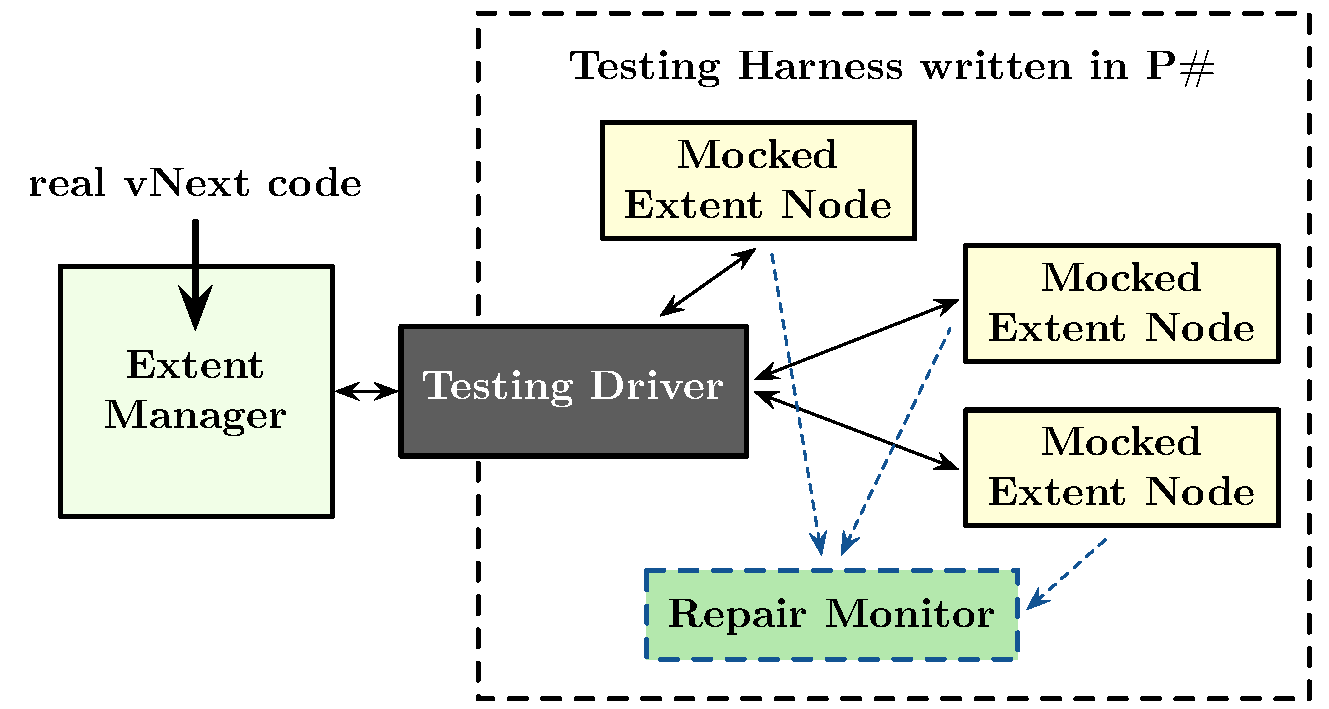
\includegraphics[width=\linewidth]{img/mocked_vnext}
\caption{Real Extent Manager with a mocked environment (each box represents one \psharp machine).}
\label{fig:azurestoremodel}
\end{figure}

\subsection{The ExtentManager machine}
\label{sec:method:wrap_target}

The real ExtMgr in vNext, which is our system-under-test, is wrapped inside the \texttt{ExtentManager} \psharp machine in the testing harness.

\begin{figure*}[t]
\centering
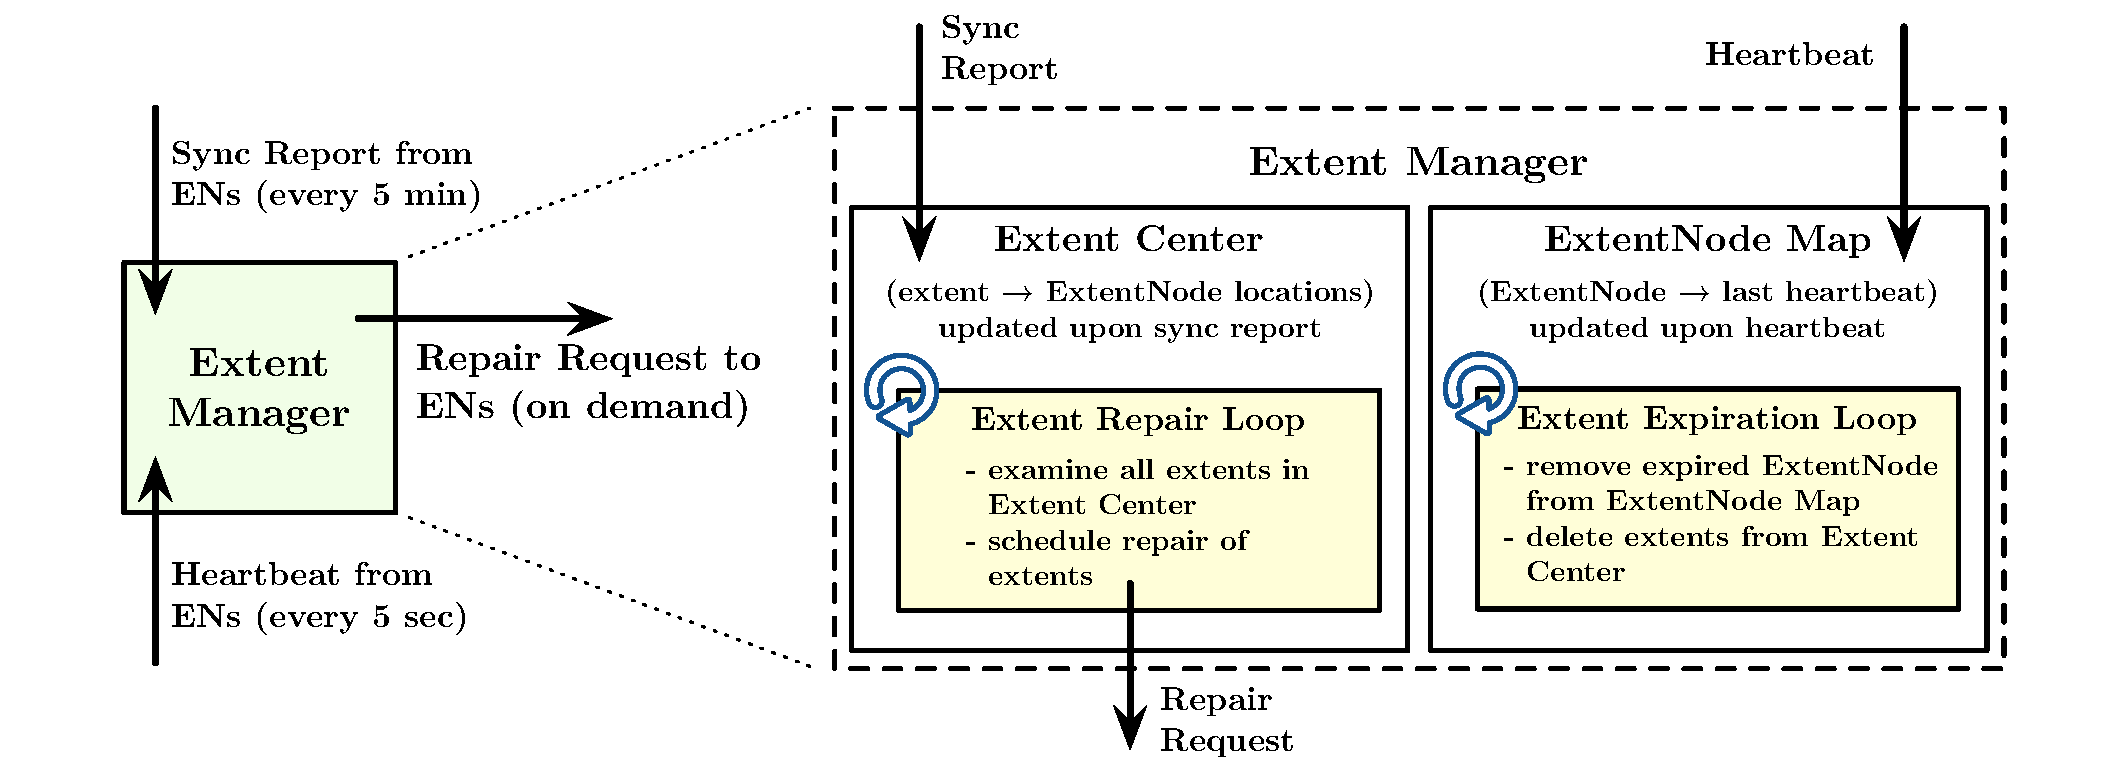
\includegraphics[width=.9\linewidth]{img/extent_manager}
\caption{Internal components of the real Extent Manager in Azure Storage vNext.}
\label{fig:extentmanager}
\end{figure*}

\textbf{Internals of the real Extent Manager}.
Inside the real ExtMgr (see Figure~\ref{fig:extentmanager}), there are two data structures related to extent replication and repair: \texttt{ExtentCenter} and \texttt{ExtentNodeMap}. The \texttt{ExtentCenter} maintains the mapping records from extents to their hosting ENs. It is updated upon the periodic sync reports from the ENs. Recall that the sync report from a particular EN lists all the extents stored at the EN. Its purpose is to update extent manager's possible out-of-date view of the EN with the ground truth. The EN map records the latest heartbeat time from every EN.

The ExtMgr runs internally a periodic {\em EN expiration loop} that is responsible for removing ENs that have been missing heartbeats for an extended period, as well as cleaning up the corresponding records in the \texttt{ExtentCenter}. In addition, the ExtMgr runs a periodic {\em extent repair loop} that examines all the \texttt{ExtentCenter} records, identifies extents with missing replicas, schedules extent repair tasks and sends them to the ENs.

\textbf{Intercepting messages between machines}.
The real ExtMgr uses a network engine to send messages to the ENs. The testing harness mocks the original network engine in vNext and overrides its interface. In this way, the mocked network engine intercepts all outbound messages and relays them to the \texttt{TestingDriver} machine, which is responsible for dispatching the messages to the corresponding \texttt{ExtentNode} machines. As shown in Figure~\ref{fig:enginecode}, the mocked network engine intercepts the outbound messages from the ExtMgr and invokes \texttt{PSharpRuntime.Send(...)} to asynchronously relay the messages to \texttt{TestingDriver}. Conceivably, the mocked network engine could leverage the nondeterminism support in \psharp and choose to drop the messages in a non-deterministic fashion, in case emulating message loss is desirable.

%Method dispatch is the process of selecting which method, from a set of available methods with the same interface, should be invoked during a program's execution. There are two types of method dispatch: \emph{static}, which is resolved during compilation; and \emph{dynamic}, which is resolved in runtime.  \csharp (and thus \psharp) supports both static and dynamic dispatch, and provide the \texttt{virtual} modifier that can be used to declare a method which can be \emph{overridden} during runtime by an inheriting class. This capability is provided by the common language runtime (CLR) of Microsoft's .NET framework, and is a key feature of \csharp as well as other mainstream object-oriented languages.

%Using method dispatch for modeling is straightforward. The system-under-test exposes a set of APIs as \emph{virtual methods}. The developer can then \emph{override} these APIs and replace them with \emph{mocks} that will execute instead of the original implementations during systematic testing with \psharp.

%\begin{figure}[t]
%\begin{lstlisting}
%// Public interface of the real network engine
%class NetworkEngine {
  %public virtual void SendMessage(Socket s, Message msg);
  %public virtual void EnqueueMessage(Message msg);
%}
%
%// The mocked network engine used during testing
%class MockedNetEngine : NetworkEngine {
  %ExtentManager EM; // Handle to actual system-under-test
  %MachineId Env; // Handle to modeled environment
  %
  %public MockedNetEngine(ExtentManager em, MachineId env) {
    %this.EM = em;
    %this.Env = env;
  %}
  %
  %public override void SendMessage(Socket s, Message msg) {
    %PSharpRuntime.Send(this.Env, new MsgEvent(), s, msg);
  %}
  %
  %public override void EnqueueMessage(Message msg) {
    %this.EM.ProcessMessage(msg);
  %}
%}
%\end{lstlisting}
%\vspace{-2mm}
%\caption{The mocked network engine used for testing the Azure Storage vNext system.}
%\label{fig:enginecode}
%%\vspace{-2mm}
%\end{figure}

\begin{figure}[t]
\begin{lstlisting}
// network interface in vNext
class NetworkEngine {
  public virtual void SendMessage(Socket s, Message msg);
}

// mocked engine for intercepting Extent Manager messages
class MockedNetEngine : NetworkEngine {
  public override void SendMessage(Socket s, Message msg) {
    // intercept and relay Extent Manager messages
    PSharpRuntime.Send(this.TestingDriver,
      new MessageFromExtentManagerEvent(), s, msg);
  }
}
\end{lstlisting}
\vspace{-2mm}
\caption{Mocked network engine in vNext.}
\label{fig:enginecode}
%\vspace{-2mm}
\end{figure}

%We now give an example of using dynamic dispatch to model the network engine of an extent manager in the Azure Storage vNext case study (see Figure~\ref{fig:enginecode}). The network engine is responsible for sending to and receiving messages from the various components of the system. During real execution, the network engine uses a custom remote procedure call (RPC) .NET library for communication. For testing, though, it is desirable to replace all calls to this RPC library with \psharp send and receive operations, which can be captured and systematically interleaved to find bugs. We easily achieved this by exposing the original send message operation of the network engine as a virtual method, and then overriding it for testing. In the overridden method, we created a \psharp event and then we wrapped the original message in this event's payload. Then, instead of invoking the RPC library, we invoke the \texttt{PSharpRuntime.Send(...)} method, which asynchronously sends the event (containing the original message) to the target extent node machine.

%For mocking the receive operation, we take advantage of the implicit receive of events in \psharp machines. When a extent node machine receives an event, an appropriate event handler is invoked, which extracts the original message from the payload and then handles it accordingly.

\textbf{Specifics of the ExtentManager machine}.
Figure~\ref{fig:wrap_target} shows code snippets from the \texttt{ExtentManager} \psharp machine. \texttt{ExtentManager} is a thin wrapper of the real ExtMgr. The mocked network engine replaces the real one in ExtMgr, intercepts all the outbound messages from ExtMgr and relays them to \texttt{TestingDriver}.

%A typical wrapper machine contains a handle (as a field) to the system component that is being wrapped (in our case the real Extent Manager object) and the event handlers are responsible for translating any received events to method calls in the real code that is being tested. The \texttt{ExtentManager} is accompanied by a mocked version of the real Network Engine class. The real Extent Manager is communicating with the outside world via remote procedure calls, but in \psharp harness we want to capture this communicating and expose it as calls to \psharp communicating primitives. This is discussed in detail in \S\ref{sec:method:model:dispath}.

%As shown in Figure~\ref{fig:wrap_target}, the \texttt{ExtentManagerMachine} is a wrapper machine and is used to connect the \psharp modeled code with the legacy \csharp code. A typical wrapper machine contains a handle (as a field) to the system component that is being wrapped (in our case the real Extent Manager object) and the event handlers are responsible for translating any received events to method calls in the real code that is being tested. The \texttt{ExtentManager} is accompanied by a mocked version of the real Network Engine class. The real Extent Manager is communicating with the outside world via remote procedure calls, but in \psharp harness we want to capture this communicating and expose it as calls to \psharp communicating primitives. This is discussed in detail in \S\ref{sec:method:model:dispath}.

\begin{figure}[t]
\begin{lstlisting}
// Wrapping the target vNext component in a P# machine
class ExtentManagerMachine : Machine {
  private ExtentManager extMgr; // real vNext code

  void Init() {
    extMgr = new ExtentManager();
    extMgr.netEngine = new MockedNetEngine(); // mock network
    extMgr.isMockingTimer = true;	 // disable internal timer
  }

  [OnEvent(MessageFromExtentNode, DeliverExtentNodeMessage)]
  void DeliverExtentNodeMessage() {
    var msg = (ExtentNodeMessage)this.Payload;
    // relay messages from Extent Node to Extent Manager
    extMgr.ProcessMessage(msg);
  }
	
  [OnEvent(TimerTick), nameof(ProcessExtentRepair))]
  void ProcessExtentRepair() {
    // extent repair loop driven by external timer
    extMgr.ProcessEvent(new ExtentRepairEvent());
  }
}
\end{lstlisting}
\vspace{-2mm}
\caption{System-under-test: instance of the real Extent Manager wrapped inside the \texttt{ExtentManager} machine.}
\label{fig:wrap_target}
%\vspace{-2mm}
\end{figure}

Messages coming from the ENs do \emph{not} go through the mocked network engine. They are delivered to the \texttt{ExtentManager} machine directly and trigger an action that invokes the messages on the internal ExtMgr with \texttt{extMgr.ProcessSingleMessage}. The benefit of this approach is that ExtMgr can be tested without modifying its code; ExtMgr is simply unaware of the testing harness and behaves as if it running in a real distributed environment and communicating with real ENs.

System correctness should \emph{not} hinge on the frequency of any individual timer. Instead, all nondeterminism due to timing-related events must be delegated to \psharp. To achieve this, all timers inside ExtMgr are disabled, and the EN expiration loop and the extent repair loop are driven instead by timers modeled in \psharp, an approach that was used in previous work~\cite{desai2015building}. The \psharp timers send nondeterministic timeout events that are controlled by the \psharp runtime. Hence, the \psharp testing engine has the freedom to schedule arbitrary interleavings between timeout events and all other regular system events.

\subsection{The ExtentNode machine}
\label{sec:method:mock_en}

The \texttt{ExtentNode} machine is a simplified version of the original EN. The machine omits much of the complex details of a real EN, and only mocks the logic necessary for the testing scenarios. This mocked logic includes: repairing an extent from its replica, and sending sync reports and heartbeat messages periodically to the \texttt{ExtentManager} machine.

The testing harness leverages components of Azure Storage vNext whenever it is appropriate. For example, the \texttt{ExtentNode} machine re-uses the \texttt{ExtentCenter} data structure, a component that is used inside a real EN for extent bookkeeping.

In the mocked extent repair logic, \texttt{ExtentNode} takes action upon receiving an extent repair request from the \texttt{ExtentManager} machine. It sends a copy request to a source \texttt{ExtentNode} machine where a replica is stored. After receiving an \texttt{ExtentCopyResponse} event from the source, it updates the internal \texttt{ExtentCenter}, as illustrated in Figure~\ref{fig:mocked_en}. 

In the mocked EN sync logic, the machine is again driven by an external timer provided by \psharp. It prepares a sync report with \texttt{extCtr.GetSyncReport(...)} and asynchronously sends the report to \texttt{ExtentManager} with \texttt{PSharpRuntime.Send(...)}.

%\begin{figure}[t]
%\begin{lstlisting}
%// Wrapping the target vNext component in P#
%class ExtentNodeMachine : Machine {
  %private ExtentNode.ExtentCenter extCtr; // real vNext component
%
	%[OnEventDoAction(typeof(RepairExtentRequestEvent), nameof(ProcessRepairExtentRequest))]
	%[OnEventDoAction(typeof(DownloadExtentRequestEvent), nameof(ProcessDownloadExtentRequestEvent))]
	%[OnEventDoAction(typeof(DownloadExtentResponseEvent), nameof(ProcessDownloadExtentResponseEvent))]
	%[OnEventDoAction(typeof(TimerTickEvent), nameof(ProcessExtentNodeSyncEvent))]
%
  %void ProcessRepairExtentRequest()
  %{
    %var source = GetRepairSourceMachine(this.Payload);
    %PSharpRuntime.Send(source, new DownloadExtentRequestEvent(), this.Payload);
  %}
%
  %void ProcessDownloadExtentRequestEvent()
  %{
	  %var destination = GetRepairDestinationMachine(this.Payload);
    %var ext_id = GetExtentID(this.Payload);
    %
		%Extent ext;
    %if (extCtr.TryGet(ext_id, out ext))
      %PSharpRuntime.Send(destination, new DownloadExtentResponseEvent(), ext);
  %}
%
  %void ProcessDownloadExtentResponseEvent()
  %{
    %var ext = (Extent)this.Payload;
    %extCtr.AddExtent(ext);
%
    %this.Monitor<RepairMonitor>(new NotifyExtentRepairCompletion(), this.NodeID);
  %}
%
  %void ProcessExtentNodeSyncEvent()
  %{
    %var sync = new ExtentNodeSync(this.NodeID);
    %extCtr.Extents.ForEach(ext =>
      %{
        %var rec = new ExtentRecord(ext.ExtentID, ext.Length, ext.Sealed);
        %sync.ExtentRecs.Add(rec);
      %});
    %PSharpRuntime.Send(this.NameNode, new NameNodeMessageEvent(), sync);
  %}
%}
%\end{lstlisting}
%\vspace{-2mm}
%\caption{Mocked Extent Node.}
%\label{fig:mocked_en}
%%\vspace{-2mm}
%\end{figure}

%\begin{figure}[t]
%\begin{lstlisting}
%// Mocking Extent Node in P#
%class ExtentNodeMachine : Machine {
  %// use real vNext component whenever appropriate
  %private ExtentNode.ExtentCenter extCtr;
%
  %[OnEventDoAction(typeof(RepairExtentRequestEvent), nameof(ProcessRepairExtentRequest))]
  %[OnEventDoAction(typeof(TimerTickEvent), nameof(ProcessExtentNodeSync))]
%
  %// extent repair logic
  %void ProcessRepairExtentRequest()
  %{
    %var source = GetRepairSourceMachine(this.Payload);
    %PSharpRuntime.Send(source, new DownloadExtentRequestEvent(), this.Payload);
  %}
  %...
%
  %// extent node sync logic
  %void ProcessExtentNodeSync()
  %{
    %var sync = new ExtentNodeSync(this.NodeID);
    %extCtr.Extents.ForEach(ext =>
      %{
        %sync.ExtentRecords.Add(new ExtentRecord(ext));
      %});
    %PSharpRuntime.Send(this.ExtentManagerMachine, new MessageFromExtentNodeEvent(), sync);
  %}
%}
%\end{lstlisting}
%\vspace{-2mm}
%\caption{Mocked Extent Node.}
%\label{fig:mocked_en}
%%\vspace{-2mm}
%\end{figure}

\begin{figure}[t]
\begin{lstlisting}
// Mocking Extent Node in P#
class ExtentNodeMachine : Machine {
  // leverage real vNext component whenever appropriate
  private ExtentNode.ExtentCenter extCtr;

  // extent repair logic
  ...
  [OnEvent(ExtentCopyResponse, ProcessExtentCopyResponse)]
  void ProcessExtentCopyResponse() {
    // extent copy response from source replica
    if (IsCopySucceeded(this.Payload)) {
      var rec = GetExtentRecord(this.Payload);
      extCtr.AddOrUpdate(rec); // update Extent Center
    }
  }

  // extent node sync logic
  [OnEvent(TimerTick, ProcessExtentNodeSync)]
  void ProcessExtentNodeSync() {
    var sync = extCtr.GetSyncReport(); // prepare sync report
    PSharpRuntime.Send(this.ExtentManagerMachine,
      new MessageFromExtentNodeEvent(), sync);
  }
}
\end{lstlisting}
\vspace{-2mm}
\caption{The mocked EN in vNext.}
\label{fig:mocked_en}
%\vspace{-2mm}
\end{figure}

\subsection{The TestingDriver machine}
\label{sec:method:driver}

The \texttt{TestingDriver} machine drives two testing scenarios. In the first scenario, it launches one \texttt{ExtentManager} and three \texttt{ExtentNode} machines, with a single extent on one of the ENs. It waits for the extent to be replicated at the other ENs. In the second scenario, it fails one of the \texttt{ExtentNode} machines and launches a new one. It waits for the extent to be repaired on the new EN. We omit illustrative code snippets due to space constraints.

\subsection{The RepairMonitor machine}
\label{sec:method:monitor}

The \texttt{RepairMonitor} machine is a \psharp liveness monitor (see \S\ref{sec:bg:bugs}) that transitions between a cold and a hot state. Whenever an extent node fails, \texttt{RepairMonitor} is notified. As soon as the number of extent replicas falls below a specified target (three replicas in the current test harness), \texttt{RepairMonitor} transitions into the hot \emph{repairing} state, where the missing replica is being repaired. Whenever a replica is repaired, the \texttt{RepairMonitor} machine is also notified. It transitions into the cold \emph{repaired} state, when the replica number reaches again the target, as illustrated in Figure~\ref{fig:monitor}.

In the extent repair testing scenarios, \texttt{RepairMonitor} checks that it should {\em always eventually} end up in the cold repaired state. Otherwise, the \texttt{RepairMonitor} machine is stuck in the hot repairing state for {\em infinitely} long. This indicates that the corresponding execution sequence results in an extent replica never being repaired, which is a liveness bug.

\begin{figure}[t]
\begin{lstlisting}
class RepairMonitor : Monitor {
  // true: EN has replica, false: EN has no replica
  private Dictionary<Machine, bool> ExtentNode2Replica;

  // cold state: repaired
  [OnEvent(NotifyEnFailure, ProcessExtentNodeFailure)]
  cold state Repaired {
    void ProcessExtentNodeFailure() {
        var node = GetExtentNode(this.Payload);
        ExtentNode2Replica.Remove(node);
        goto Repairing;
    }
  }

  // hot state: repairing
  [OnEvent(NotifyExtentRepaired, ProcessExtentRepaired)]
  hot state Repairing {
    void ProcessExtentRepaired() {
      var node = GetExtentNode(this.Payload);
      ExtentNode2Replica[node] = true;
      if (ReplicaCount == Harness.REPLICA_COUNT_TARGET)
        goto Repaired;
    }
  }
}
\end{lstlisting}
\vspace{-2mm}
\caption{The RepairMonitor machine.}
\label{fig:monitor}
%\vspace{-2mm}
\end{figure}

\subsection{Liveness Bug in Azure Storage vNext}
\label{sec:method:azurestore}

It took less than ten seconds for the \psharp testing engine to report the first occurrence of a liveness bug in vNext (see \S\ref{sec:eval}). Upon examining the debug trace, the developers of vNext were able to quickly confirm the bug.

However, the original \psharp trace did not include sufficient detail to allow the developers to identify the root cause of the problem. Fortunately, running the test harness took very little time, so the developers were able to quickly iterate and add more refined debug outputs in each iteration. After several iterations, the developers were able to pinpoint the exact culprit and immediately propose a solution for fixing the bug. Once the proposed solution was implemented, the developers ran again the test harness. No bugs were found during 100,000 iterations, a process that required only tens of minutes.

The liveness bug occurs in the second testing scenario, where the \texttt{TestingDriver} fails one of the \texttt{ExtentNode} and launches a new one. The \texttt{RepairMonitor} transitions to the hot repairing state and is stuck in the state for infinitely long.

The following is one particular execution sequence resulting in this liveness bug: (i) EN$_0$ fails and is detected by the EN expiration loop; (ii) EN$_0$ is removed from the EN map; (iii) the extent center is updated and the replica count drops from 3 (which is the target) to 2; (iv) ExtMgr receives a sync report from EN$_0$; (v) the extent center is updated and the replica count increases again from 2 to 3. This is problematic since the replica count is equal to the target, which means that the extent repair loop will never schedule any repair task. At the same time, there are only two \emph{true} replicas in the system, which is one less than the target. This execution sequence leads to one missing replica; repeating this process two more times would result in all replicas missing, but ExtMgr still thinking that all replicas are healthy. In production, such a bug can cause a very serious incident of customer data loss.

The culprit is in (iv), where ExtMgr receives a sync report from EN$_0$ after deleting the EN. This may occur in \psharp due to arbitrary interleaving of events. It may also occur, albeit much less frequently, during stress testing due to messages being delayed in the network. This explains why the bug only occurs from time to time during stress testing and requires long executions to manifest. In contrast, \psharp allows the bug to manifest quickly, the developers to iterate rapidly, the culprit to be identified promptly, and the fix to be tested effectively and thoroughly, all of which have the potential to vastly increase the productivity of distributed storage system development.

%%\subsection{Modeling the environment}
%\subsection{Test Harness}
%\label{sec:method:model}
%
%The environment of a distributed system might consist of other distributed systems and services, clients, operating system timers, as well as libraries for networking or other purposes. To be able to systematically test a distributed system, this environment must be modeled and all the interactions between the environment and the system, as well as all the nondeterminism, must be captured and controlled by the \psharp runtime.
%
%%\subsubsection{Creating a test harness using \psharp}
%\subsubsection{Orchestrating Machines}
%\label{sec:method:model:harness}
%
%\begin{figure}[t]
%\centering
%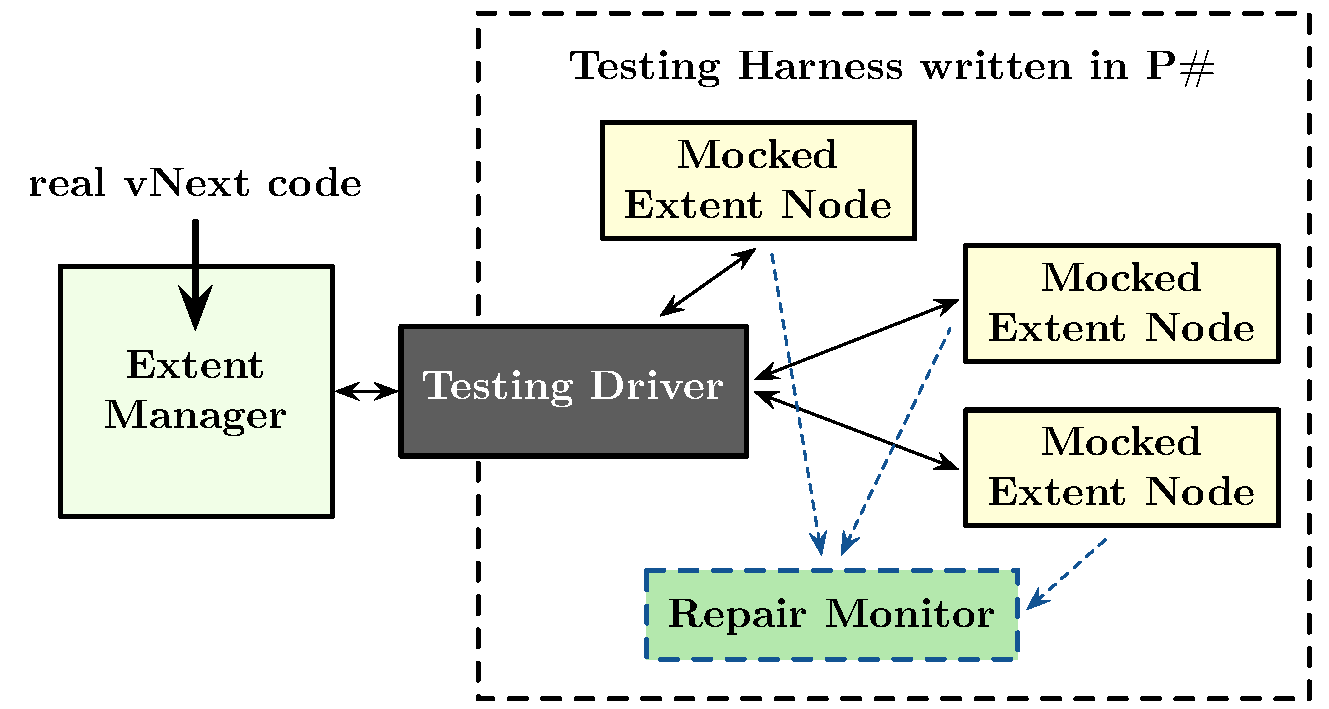
\includegraphics[width=\linewidth]{img/mocked_vnext}
%\caption{The real environment of the Extent Manager is replaced with a mocked version for testing.}
%\label{fig:azurestoremodel}
%\end{figure}
%
%Before being able to use \psharp to test an existing distributed system, the environment of the components that the developer wants to test have to be modeled using the \psharp state machine APIs.  This involves creating mock classes that inherit from the \texttt{Machine} abstract class. The \texttt{Machine} class exposes methods for declaring a state machine (e.g. machine states and state transitions) as well as methods for sending events to other machines, declaring event handlers for received events, and accessing the payload from the latest received event.
%
%In the Azure Storage vNext case study, we created the following \psharp machines: \texttt{Environment}, \texttt{ExtentNode}, \texttt{ExtentManager}, and \texttt{Timer}.
%
%The \texttt{Environment} (denoted with a dashed line box in Figure~\ref{fig:azurestoremodel}) is essentially a ``god'' machine: it is the very first machine that is created; has a handle to all other machines in the harness; and includes the logic based on which the test harness will execute. The programmer is free to create either a finite test harness (e.g. with a predefined number of node failures) or an infinite test harness (e.g. with an unbounded number of failures), as long as any nondeterminism (e.g. when to insert a failure) is captured using the available \psharp APIs.
%
%Finally, the \texttt{Timer} machine models the operating system timer and is responsible for triggering events related to the Azure Storage vNext logic (e.g. synchronization messages, heartbeats and repair logic loops). This is discussed in detail in \S\ref{sec:method:model:timers}.
%
%\subsubsection{Modeling and injecting failures}
%\label{sec:method:model:failures}
%
%In production, each Extent Node of the Azure Storage vNext system periodically (every 5 seconds) sends a heartbeat to the Extent Manager which notifies that the Extent Node is alive. Because we want to model failures and systematically inject them using \psharp, we abstract away the heartbeat mechanism in our harness. However, the Extent Manager logic relies on time intervals to detect node failures (see Figure~\ref{fig:expiration}). The way to abstract this time-related logic and connect the real code with the modeled code is to use virtual dispatch and override the virtual \texttt{IsNodeExpired} method with a mocked version.
%
%\begin{figure}[t]
%\begin{lstlisting}
%// Real code for detecting node expiration
%public virtual bool IsNodeExpired(string id, DateTime time)
%{
  %return DateTime.Compare(time, DateTime.Now) <= 0;
%}
%
%// Mocked code for detecting node expiration
%public override bool IsNodeExpired(string id, DateTime time)
%{
  %return this.DeletedNodes.Contains(id);
%}
%\end{lstlisting}
%\vspace{-2mm}
%\caption{Abstracting the node expiration logic in the Extent Manager component of Azure Storage vNext.}
%\label{fig:expiration}
%%\vspace{-2mm}
%\end{figure}
%
%Figure~\ref{fig:expiration} presents how we mocked the node expiration detection method. Instead of comparing the time interval as in the original code, we now check if the set \texttt{DeletedNodes} contains the id of the Extent Node that we are checking for expiration. If it contains the id, then it means that the node has failed. The \texttt{Environment} machine that we have created as part of our testing \psharp harness, will nondeterministically choose a node to kill, then send the id of this killed node to the Extent Manager wrapper machine, who will in turn add it to the \texttt{DeletedNodes} set.
%
%\subsubsection{Entry point to a \psharp test harness}
%\label{sec:method:model:entrypoint}
%
%A developer can specify the entry point of a \psharp test harness similar to how unit tests are typically written. Figure~\ref{fig:entrypoint} shows the source code of the entry point for the Azure Storage vNext \psharp test harness. The programmer can declare an entry point method using the \texttt{Microsoft.PSharp.Test} attribute. When the \psharp systematic testing engine is invoked, it will scan the binary and attempt to find a static method declared with this attribute. When such a method is found (in our example the \texttt{Execute()} method), the testing engine will invoke it and start testing the program. The systematic engine can optionally run multiple iterations of the test harness, each one potentially exploring a different schedule. In each iteration, the program state will be reset (any static fields must be explicitly reset by the programmer) and the entry point will be re-invoked.
%
%\begin{figure}[t]
%\begin{lstlisting}
%[Microsoft.PSharp.Test]
%public static void Execute()
%{
  %PSharpRuntime.CreateMachine(typeof(Environment));
%}
%\end{lstlisting}
%\vspace{-2mm}
%\caption{Static \csharp method acting as the entry point to the Azure Storage vNext \psharp test harness.}
%\label{fig:entrypoint}
%%\vspace{-2mm}
%\end{figure}
%
%\subsubsection{Abstracting timers}
%\label{sec:method:model:timers}
%
%Distributed systems are often using timers to determine when an event should be send from one component to another. For example, in the Azure Storage vNext system, each Extent Node is associated with a timer that fires of a synchronization message every 5 minutes and a heartbeat every 5 seconds. This timer is related to the liveness bug that we discovered: the synchronization message that gets fired every 5 minutes can potentially race with an Extent Node failure; if it arrives after the node failed, then the bug would manifest. Traditional testing techniques cannot easily find such a bug, due to the very infrequent occurrence of this race due to the timer. 
%
%Our methodology in \psharp to systematically test distributed systems that rely on timers, is to abstract timers away, model them using message passing communication and introduce nondeterminism in their firing. This nondeterminism is introduced using the \psharp \texttt{Nondet()} method, which returns a nondeterministic boolean value that is controlled by the \psharp runtime during systematic testing.
%
%Figure~\ref{fig:timer} shows how we modeled a generic timer in the Azure Storage vNext case study. The Extend Manager, as well as each Extent Node in the harness, is associated with a unique \texttt{Timer} machine. When creating this machine, we pass as a payload the id of the machine that owns this timer. When the \texttt{Timer} machine is created, it stores this id in the \texttt{Owner} field and then transitions to the \texttt{Active} state. In this state, the \texttt{Timer} loops infinitely and nondeterministically (using \texttt{Nondet()}) sends a \texttt{TimerTickEvent} to \texttt{this.Owner}. When the Extent Node owner receives this event, it handles it by generating a synchronization message that is being send to the Extent Manager. Similarly, when the Extent Manager receives a \texttt{TimerTickEvent} from its own \texttt{Timer}, it handles it by nondeterministically invoking repair-related methods in the Extent Repair Center data structure. 
%
%\begin{figure}[t]
%\begin{lstlisting}
%internal class Timer : Machine
%{
  %MachineId Owner; // Id of the owner machine
%
  %[Start]
  %[OnEntry(nameof(InitOnEntryAction))]
  %[OnEventGotoState(typeof(Unit), typeof(Active))]
  %class Init : MachineState { }
%
  %void InitOnEntryAction()
  %{
    %this.Owner = (MachineId)this.Payload;
    %// triggers state transition to Active
    %this.Raise(new Unit());
  %}
%
  %[OnEntry(nameof(ProcessTickEvent))]
  %[OnEventGotoState(typeof(Unit), typeof(Active))]
  %class Active : MachineState { }
%
  %void ProcessTickEvent()
  %{
    %// Nondeterministic boolean choice controlled by P#
    %if (this.Nondet())
      %// sends a timer tick event to the owner machine
      %this.Send(this.Owner, new TimerTickEvent());
    %// triggers state transition to Active
    %this.Raise(new Unit());
  %}
%}
%\end{lstlisting}
%\vspace{-2mm}
%\caption{Timers in Azure Storage vNext are modeled as nondeterministic \psharp machines.}
%\label{fig:timer}
%%\vspace{-2mm}
%\end{figure}


\section{Case studies}
\label{sec:cases}

% cheng to review
\subsection{Distributed Extent Management System}
\label{sec:cases:azurestore}

We used \psharp to test the \emph{distributed extent management} component of the Windows Azure vNext distributed storage system. This component is responsible for managing the partitioned extent metadata and works as follows.

There are multiple \emph{extent managers} (EMgrs) that are in charge of managing a subset of the extents. Each EMgr communicates asynchronously (via remote procedure calls) with a number of \emph{extent nodes} (ENs) that store the extents. Each EN sends: (i) a \emph{heartbeat} every 5 seconds, to notify the EMgr that it is still available; and (ii) a \emph{sync report} every 5 minutes, to synchronize its extent with the rest of the nodes. The EMgr contains two data structures: an \emph{extent center} (ECtr), which is updated every time an EN syncs; and an EN map, which is updated every time it receives a heartbeat from an EN. The EN map runs an EN expiration loop that is responsible for removing ENs that have expired from the EN map and also delete them from the ECtr. Finally, the EMgr runs an extent repair loop, which examines all contents of all extents in the ECtr and schedules repairs of extents if they are out-of-date (via a repair request).

\subsection{Live Azure Table Migration}

We also used \psharp to test the MigratingTable library, which is capable of transparently migrating a data set between tables in the Windows Azure storage service while an application is accessing the data set.  MigratingTable provides a ``virtual table'' with an API similar to that of an ordinary Azure table, backed by a pair of ``old'' and ``new''  tables.  It moves all data from the old table to the new table in the background.  Meanwhile, each read or write issued to the virtual table is translated to a sequence of reads and writes on the backend tables according to a protocol we designed, which guarantees linearizability of operations on the virtual table across multiple application processes assuming that the backend tables respect their own linearizability guarantees.

% N.B. Artifact Services is mentioned at http://research.microsoft.com/en-us/people/schulte/.  Hopefully it's OK to reveal that it was the system in this case study. ~ Matt 2015-08-17
The initial motivation for MigratingTable was to solve a scaling problem for Artifact Services, an internal Microsoft system with a data set that is sharded across tables in different Azure storage accounts because of the limit on traffic supported by a single Azure storage account.  As the traffic continues to grow over time, we will need to reshard the data set across a greater number of Azure storage accounts without interrupting service.  During such a resharding, our sharding manager will identify each key range that should migrate to a different table, and we will use a separate MigratingTable instance for each such key range to actually perform the migration.  MigratingTable may also be useful to migrate data to a table with different values of configuration parameters that Azure does not support changing on an existing table, such as geographic location.

Since we were designing a new concurrent protocol that we expected to become increasingly complex over time as we add optimizations, we planned from the beginning to maintain a \psharp test harness along with the protocol to maintain confidence in its correctness.

\subsubsection{Modeling approach}
% TBD where this ends up in the paper ~ Matt 2015-08-17

MigratingTable implements an interface called IChainTable2, which provides the core read and write functionality of the real Azure table API with one exception: it provides a weaker consistency property for multi-page reads, since the original property would have been difficult to achieve for no benefit to applications we could foresee.  MigratingTable requires that its backend tables also implement IChainTable2, and we wrote a simple adapter to expose physical Azure tables as IChainTable2.  Our goal was then to verify that when multiple application processes issue ``input'' read and write calls to their own MigratingTable instances backed by the same tables, the behavior is compliant with the specification of IChainTable2 for the combined input history.

% N.B. SpecTable = InMemoryTableWithHistory in the current codebase. ~ Matt 2015-08-17
Since the specification is deterministic under sequential calls except for the results of multi-page reads, we decided the easiest way to formulate it for automated testing was to write an in-memory reference implementation called SpecTable.  Given a multi-page read, SpecTable can actually produce a list of all valid results.  Our correctness property is then:
\begin{quote}
For every execution trace of a collection of MigratingTables backed by the same pair of SpecTables (which nondeterministically choose one of the valid results for each multi-page read), there exists a linearization of the combined input history such that the output in the original trace matches the output of a ``reference'' SpecTable on the linearized input.
\end{quote}
%
\def\term#1{\emph{#1}}
We instrumented MigratingTable to report the \term{linearization point} of each input call, which in our case is always one of the corresponding \term{backend calls} to the backend tables (often the last).  Specifically, after each backend call, MigratingTable reports whether it was the linearization point, which may depend on the result of the call.  This makes it possible to verify the correctness property as the system executes.  We have a \term{tables machine} containing all three SpecTables and a collection of \term{service machines} each containing a MigratingTable.  Each service machine issues a random sequence of input calls to its MigratingTable, which sends backend calls to the tables machine.  When MigratingTable reports the linearization point of an input call, the service machine sends that input call to the reference table.  When an input call completes, the service machine checks that the results from the MigratingTable and the reference table agree.  \psharp controls the interleaving of the backend calls.  After the tables machine processes a backend call, it enters a state that defers further backend calls until MigratingTable has reported whether the backend call was a linearization point and (if so) the call to the reference table has been made.  We use the \psharp nondeterminism API to generate the input calls, so in principle an exhaustive \psharp behavior exploration strategy such as DFS could be used to exhaustively test MigratingTable up to some bound.

% Draft
We wanted to implement the core MigratingTable algorithms in \csharp ``async'' code, like most of Artifact Services.  Async code is readable like traditional procedural code but is translated by the compiler to an event-driven state machine using the Task Parallel Library, gaining most of the performance benefits of that style.  By default, all event processing occurs on the .NET thread pool.

We had to arrange for the continuations to execute within the context of a single \psharp machine, which we did by installing a custom SynchronizationContext.  Then we implemented async RPC between machines in terms of message passing, using RealProxy to avoid most of the marshaling boilerplate.

\section{Evaluation}
\label{sec:eval}

Paragraph that says what will be discussed in evaluation and what are the results (very short)

\subsection{Experimental Setup}

\subsection{Benchmarks}

Benchmarks that are not production code (e.g. multipaxos) that can be used to evaluate testing

Cheng's case study with the actual bug

Matt's case study with injected bugs

\subsection{Stressing testing vs Systematic testing}

Comparison of traditional stress testing VS what we do with \psharp

How long you had to run the test to find the bug (if you can find it) and how long are the traces

How easy it is to pinpoint the error using the \psharp traces, comparing to traditional stress testing

Effort required to use the system

\section{Related Work}
\label{sec:rw}

\psharp is most closely related to \textsc{MoDist}~\cite{yang2009modist}, a model checker that can be applied on unmodified distributed systems. To achieve this, the tool uses binary instrumentation (reuses the instrumentation engine of the D$^3$S testing tool) to expose all actions of the system under test, and then uses a model checking engine to systematically explore these actions. \textsc{MoDist} also provides a virtual clock manager that can simulate timeouts and accelerate the passage of time. A major limitation of \textsc{MoDist} is that it must be applied on a whole system, which does not scale for production systems. In contrast, \psharp has built-in support for modeling the environment of individual components of a system, which allows the tool to achieve scalability. Further, \psharp is an extension of the \csharp language and has built-in systematic testing support; it does not need to perform binary instrumentation which can be computationally expensive.

\textsc{MaceMc}~\cite{killian2007life} is a model checker for distributed systems implemented in the \textsc{Mace} language. The focus of \textsc{MaceMc} is to find liveness property violations using an algorithm based on bounded random walk and the use of heuristics. \psharp differs from \textsc{MaceMc} in that it can be applied on legacy code written in a mainstream language, whereas a system to be tested with \textsc{MaceMc} has to be written in \textsc{Mace}, which makes \textsc{MaceMc} harder to be applied in an industrial setting. Further, \psharp uses a simpler, but effective, algorithm for detecting liveness bugs.

\textsc{Fate} and \textsc{Destini} is a framework for systematically injecting (combination of) failures in distributed systems~\cite{gunawi2011fate}. This framework focuses in exercising failure scenarios, whereas \psharp can be used for testing generic safety and liveness properties of distributed systems. \psharp also provides language extensions and modeling capabilities that further differentiate it from prior work.

DieCast~\cite{gupta2008diecast}

A completely different approach for reasoning about the correctness of distributed systems is to use formal methods.  A notable example is TLA+~\cite{lamport1994temporal}, a formal specification language that can be used to design and verify concurrent programs via model checking. Amazon recently published an article describing their use of TLA+ in Amazon Web Services to verify distributed protocols~\cite{newcombe2015aws}. A limitation of TLA+, as well as other similar specification languages, is that they are applied on a model of the system and not the actual system. Even if the model is verified, the gap between a real-world implementation and the verified model is still significant, so implementation bugs are still a realistic concern.

Another approach is Verdi~\cite{wilcox2015verdi}, where a distributed system is written and verified in Coq, and then OCaml code is produced for execution. Verdi cannot find liveness bugs. \psharp is also more production-friendly: it works on \csharp, which is a mainstream language.


\section{Conclusion}
\label{sec:concl}

Draft.

%\section{Acknowledgments}
%Draft.

%
% The following two commands are all you need in the
% initial runs of your .tex file to
% produce the bibliography for the citations in your paper.
\bibliographystyle{abbrv}
\bibliography{references}  % sigproc.bib is the name of the Bibliography in this case
% You must have a proper ".bib" file
%  and remember to run:
% latex bibtex latex latex
% to resolve all references
%
% ACM needs 'a single self-contained file'!
%
%APPENDICES are optional
%\balancecolumns

\end{document}
